% Gerado de tcc.md (exportado do Claude Docs) por ferramentas/gera_latex.php em 12/11/2026 21:45.
% Para mudar o texto, edite este arquivo; se gerar de novo a partir do documento, as edições feitas aqui se perdem.

\chapter{O SISTEMA UNIA}\label{cap:4}

O UNIA é uma aplicação web em que o professor cadastra alunos, registra o estudo de caso e as metas do PEI, aplica sessões de mini games na tela e acompanha a evolução de cada meta. Este capítulo descreve os requisitos, a arquitetura, o modelo de dados, os mini games, as regras de medição, os gráficos, a segurança e a acessibilidade do sistema.

\section{Visão geral e requisitos}\label{sec:4.1}

O sistema tem dois perfis de conta: o professor, que acompanha os próprios alunos, e o administrador, que também mantém a lista de tipos de deficiência. O aluno não tem conta: ele responde às sessões no dispositivo do professor, dentro da sessão aberta por este. O uso típico segue seis passos:

\begin{passos}
  \item O professor cria a conta e entra no sistema.
  \item Cadastra o aluno, com o estudo de caso, o tipo de deficiência, quando informado, e o registro do consentimento do responsável.
  \item Cria as metas do PEI: área, habilidade, nível de suporte inicial e data de revisão.
  \item Escolhe os mini games na ficha do aluno, ou aceita uma sugestão, e entrega o dispositivo ao aluno.
  \item O aluno responde às rodadas, e o sistema grava o resultado na meta.
  \item O professor acompanha a evolução da meta e revisa o plano na data prevista.
\end{passos}

Os Quadros~\ref{qua:4} e~\ref{qua:5} listam os requisitos funcionais (RF) e não funcionais (RNF).

\begin{tabelaIFTO}
\setlength{\largtab}{\dimexpr\linewidth-4\tabcolsep-3\arrayrulewidth-1pt\relax}
\begin{longtable}{|L{0.16}|L{0.84}|}
\legendatab{quadro}{Requisitos funcionais}{qua:4}{2}\\
\hline
\textbf{Código} & \textbf{Requisito} \\
\hline
\endfirsthead
\multicolumn{2}{@{}r@{}}{\textit{(continuação)}}\\
\hline
\textbf{Código} & \textbf{Requisito} \\
\hline
\endhead
\multicolumn{2}{@{}r@{}}{\textit{(continua)}}\\
\endfoot
\fontetab{2}{elaboração própria (2026).}
\endlastfoot
RF01 & Cadastrar professor, entrar e sair do sistema e recuperar a senha por e-mail. \\ \hline
RF02 & Manter os dados da conta, trocar a senha e excluir a própria conta. \\ \hline
RF03 & Cadastrar, editar, listar, buscar e excluir alunos, com estudo de caso, tipo de deficiência e registro do consentimento do responsável. \\ \hline
RF04 & Cadastrar metas do PEI por área, com habilidade, nível de suporte inicial, professor responsável e data de revisão (padrão de 90 dias). \\ \hline
RF05 & Manter o catálogo de atividades, com busca, filtros por tipo de deficiência e por área, paginação, imagem, vídeo, fonte e mini game obrigatório. \\ \hline
RF06 & Sugerir, para cada meta, atividades da mesma área ainda não aplicadas ao aluno e compatíveis com o tipo de deficiência dele. \\ \hline
RF07 & Executar sessões de mini games na tela, com dica e cancelamento, e gravar um registro por meta. \\ \hline
RF08 & Calcular e exibir, por meta, os indicadores de evolução e os gráficos. \\ \hline
RF09 & Exibir o histórico de sessões, com o detalhe por jogo, e permitir excluir um registro feito por engano. \\ \hline
RF10 & Avisar, na tela inicial, as metas com data de revisão vencida. \\ \hline
RF11 & Permitir ao administrador manter os tipos de deficiência. \\ \hline
\end{longtable}
\end{tabelaIFTO}

\begin{tabelacurta}
\setlength{\largtab}{\dimexpr\linewidth-4\tabcolsep-3\arrayrulewidth-1pt\relax}
\legenda{quadro}{Requisitos não funcionais}\label{qua:5}\vspace{4pt}
\begin{tabular}{|L{0.1553}|L{0.8447}|}
\hline
\textbf{Código} & \textbf{Requisito} \\
\hline
RNF01 & Segurança: senhas com hash, consultas parametrizadas, proteção contra CSRF e Cross-Site Scripting (XSS) e controle de acesso por perfil e por dono do dado. \\ \hline
RNF02 & Privacidade: cada professor vê apenas os próprios alunos, e o cadastro registra o consentimento do responsável. \\ \hline
RNF03 & Acessibilidade: práticas inspiradas nas Web Content Accessibility Guidelines (WCAG) 2.1, alvos de toque de pelo menos 44 px e nenhuma informação transmitida só por cor. \\ \hline
RNF04 & Uso em tablet: as sessões funcionam por toque, com botões grandes. \\ \hline
RNF05 & Portabilidade: o sistema roda em servidor PHP com MySQL ou MariaDB, em qualquer pasta do servidor. \\ \hline
RNF06 & Manutenibilidade: código organizado em MVC, com as regras de medição isoladas e cobertas por testes automatizados. \\ \hline
\end{tabular}
\fonte{elaboração própria (2026).}
\end{tabelacurta}

\section{Arquitetura}\label{sec:4.2}

O UNIA segue o padrão MVC, que separa os dados e as regras (Model), a apresentação (View) e o controle do fluxo da requisição (Controller), e o padrão \textit{Front Controller}, em que um único ponto de entrada recebe todas as requisições (FOWLER, 2006). A Figura~\ref{fig:1} mostra a organização do código num diagrama de pacotes da UML.

\begin{figure}[hbp]
  \legendafig{figure}{Diagrama de pacotes do UNIA}{fig:1}
  % Diagrama de pacotes da UML com public, config, core e app (Controllers, Models, Services e Views), ligados por dependências «use» e «instantiate»
  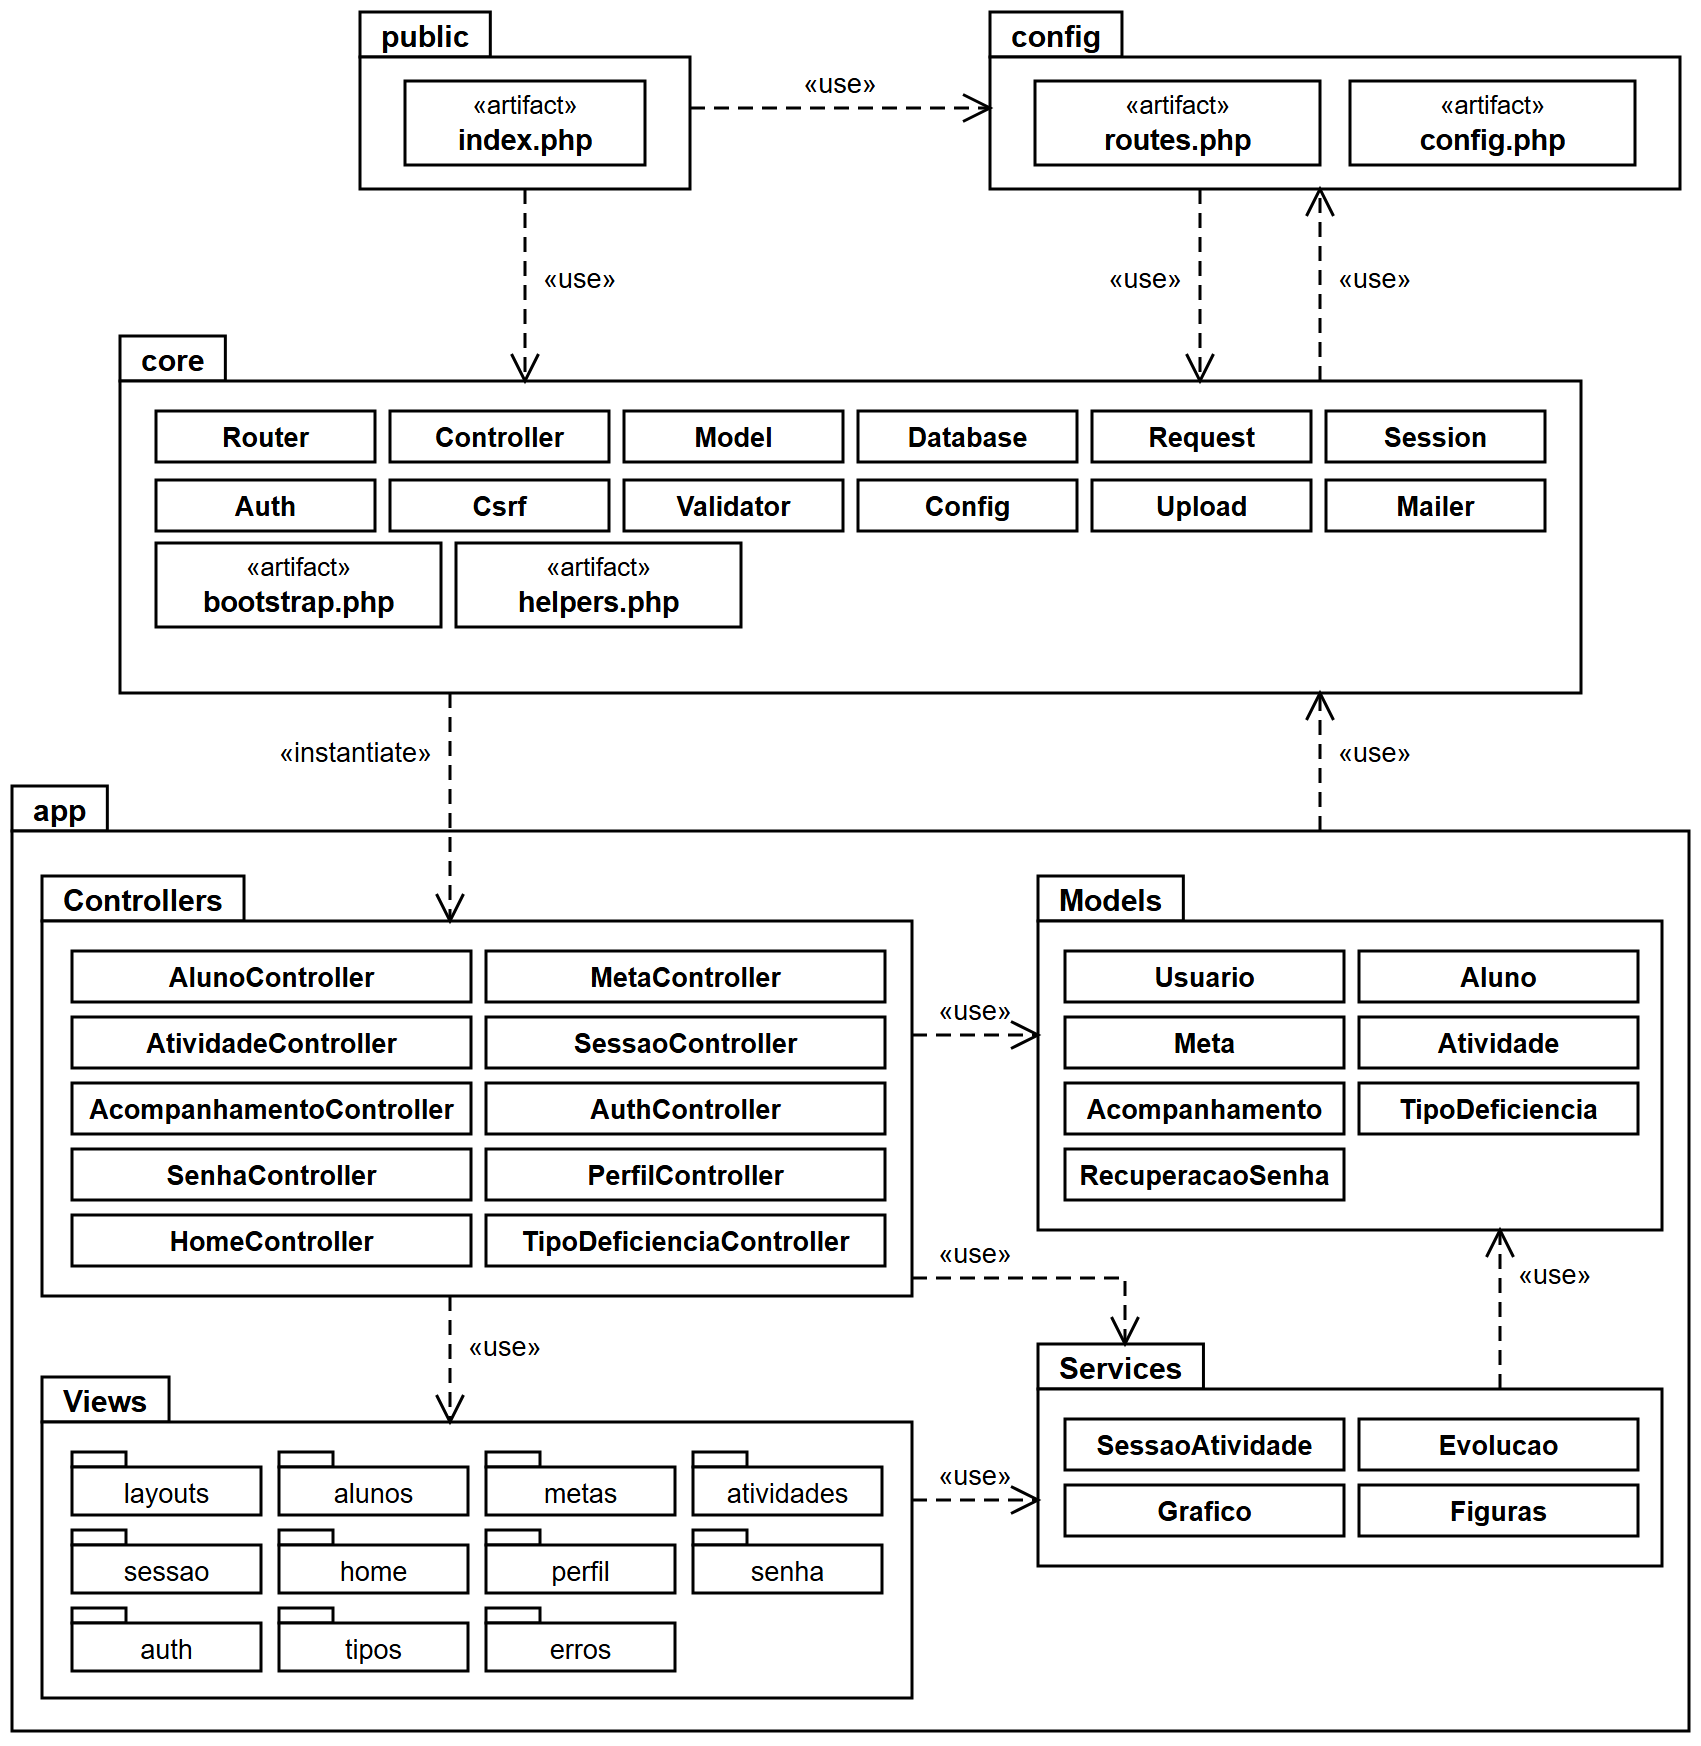
\includegraphics[width=15cm,height=17cm,keepaspectratio]{figuras/figura01-pacotes.png}
  \fonte{elaboração própria (2026).}
\end{figure}

Na notação da UML (OBJECT MANAGEMENT GROUP, 2017, p. 39, 248 e 657), cada pasta do projeto é um pacote, desenhado como um retângulo com uma aba; como os elementos do pacote aparecem dentro dele, o nome fica na aba. As classes aparecem só com o nome, e os arquivos que não são classes, como \textit{index.php} e \textit{routes.php}, aparecem como artefatos, com a palavra-chave «artifact». Cada seta tracejada é uma dependência: o pacote de onde ela sai precisa do pacote para onde ela aponta. A palavra-chave «use» indica que um pacote usa elementos do outro, e «instantiate», que cria instâncias deles, como faz o roteador do núcleo ao criar o controlador de cada requisição. Os pacotes \textit{core} e \textit{config} dependem um do outro, porque \textit{routes.php} cria o roteador e a classe \textit{Config} lê \textit{config.php}. A seta que sai de \textit{app} resume as dependências dos controladores, dos modelos e das views em relação ao núcleo; dependências menores, como a leitura de constantes dos modelos pelas views, foram omitidas para não poluir a figura.

O servidor Apache encaminha para \textit{public/index.php} toda requisição que não seja de um arquivo real, como uma folha de estilo ou uma imagem; esse arquivo carrega o núcleo e entrega a requisição ao roteador. O roteador associa o método do Hypertext Transfer Protocol (HTTP) e o endereço, ou Uniform Resource Locator (URL), a uma ação de um controlador, aplica as verificações de acesso (visitante, usuário logado ou administrador) e, em toda requisição POST, confere o token contra CSRF antes de executar a ação. O controlador lê e valida os dados, chama os modelos, que executam os comandos em Structured Query Language (SQL), e os serviços, que fazem os cálculos, e por fim monta a tela com a view dentro do layout. Só a pasta \textit{public} fica acessível pela web; o restante do projeto fica fora do alcance do navegador.

O código se divide em núcleo (pasta \textit{core}: roteador, validação, sessão, autenticação, proteção contra CSRF e acesso ao banco, envio de e-mail e upload de imagens), controladores, modelos, que contêm apenas SQL com parâmetros, serviços e views. Os quatro serviços cuidam da montagem e da classificação das sessões (\textit{SessaoAtividade}), dos indicadores de evolução (\textit{Evolucao}), dos gráficos (\textit{Grafico}) e das figuras dos jogos (\textit{Figuras}).

As regras de medição ficam nos serviços e não dependem do banco de dados. Por isso podem ser testadas isoladamente, e o mesmo código que produz os números da tela é o que os testes conferem. O sistema tem 45 rotas, listadas no Apêndice A.

\section{Modelo de dados}\label{sec:4.3}

O banco de dados tem oito tabelas, ligadas por chaves estrangeiras, com codificação \textit{utf8mb4}. A Figura~\ref{fig:2} apresenta o modelo lógico do banco, com as tabelas, as chaves e a cardinalidade de cada relacionamento.

\begin{figure}[hbp]
  \legendafig{figure}{Modelo lógico do banco de dados do UNIA}{fig:2}
  % Modelo lógico do banco em notação pé de galinha com as oito tabelas do UNIA, chaves primárias e estrangeiras e a cardinalidade de cada relacionamento
  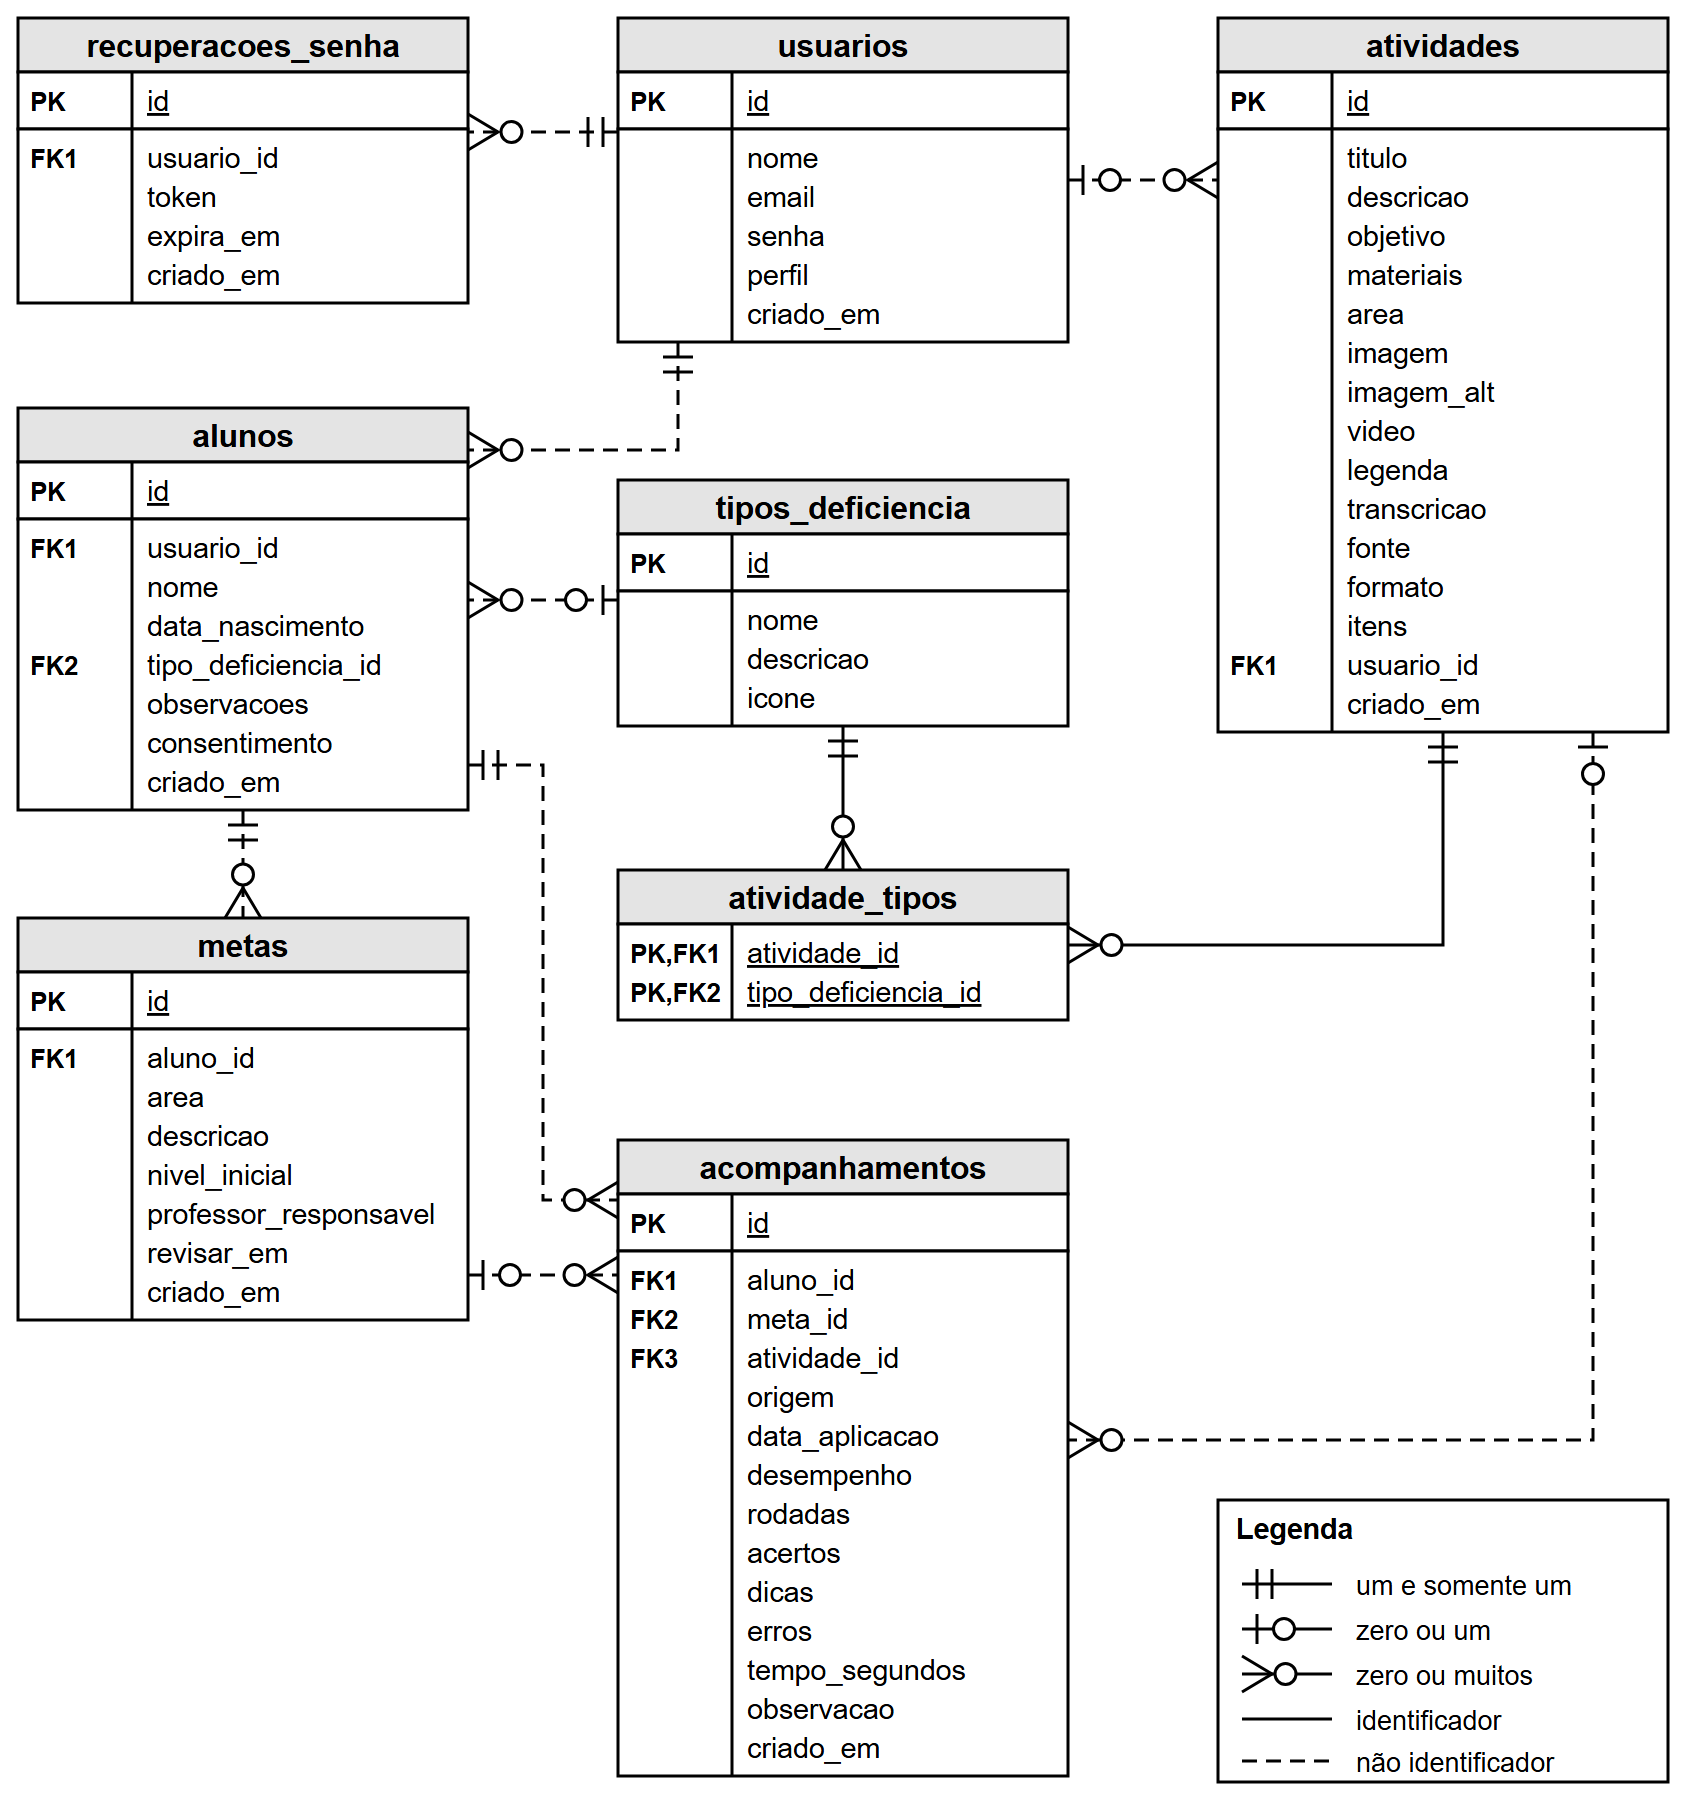
\includegraphics[width=15cm,height=17cm,keepaspectratio]{figuras/figura02-modelo-logico.png}
  \fonte{elaboração própria (2026).}
\end{figure}

O modelo usa a notação pé de galinha, no estilo dos exemplos do Apêndice A de Watt e Eng (2014, p. 129-130). Cada tabela traz o nome no cabeçalho, a chave primária (PK) sublinhada na primeira faixa e as chaves estrangeiras (FK), marcadas como FK1, FK2 e FK3. Os símbolos nas pontas das linhas dão a cardinalidade: dois traços significam um e somente um; um traço e um círculo, zero ou um; o pé de galinha com um círculo, zero ou muitos. Assim, um usuário tem zero ou muitos alunos, e cada aluno pertence a exatamente um usuário; já uma atividade pode não ter usuário, porque \textit{usuario\_id} aceita valor nulo.

A linha contínua marca o relacionamento identificador, em que a chave estrangeira faz parte da chave primária da tabela dependente (WATT; ENG, 2014, p. 41), caso das duas ligações de \textit{atividade\_tipos}; a linha tracejada marca os demais. As tabelas estão dispostas pelas ligações: \textit{usuarios} fica no alto, entre \textit{recuperacoes\_senha} e \textit{atividades}, e \textit{acompanhamentos} fica embaixo, junto das três tabelas de que depende (\textit{alunos}, \textit{metas} e \textit{atividades}). Os nomes de tabelas e colunas seguem um só padrão, o do script SQL: português, letras minúsculas e palavras separadas por sublinhado.

A tabela \textit{usuarios} guarda professores e administradores, com a senha em hash, e \textit{recuperacoes\_senha} guarda os pedidos de nova senha, com o hash do token enviado por e-mail e o prazo de validade. A tabela \textit{tipos\_deficiencia} começa com sete tipos (motora, intelectual, auditiva, visual, TEA, múltipla e “outra / não sei dizer”) e se liga às atividades por \textit{atividade\_tipos}, numa relação muitos-para-muitos. Em \textit{atividades} ficam a área, o formato do mini game, a fonte, obrigatória, e um campo opcional de configuração em JavaScript Object Notation (JSON), descrito na seção~\ref{sec:4.4}.

As três tabelas centrais do acompanhamento são \textit{alunos}, \textit{metas} e \textit{acompanhamentos}. O aluno pertence a um professor e guarda o estudo de caso e o registro do consentimento do responsável. A meta pertence a um aluno e registra a área, a habilidade priorizada, o nível de suporte inicial, o professor responsável e a data de revisão. Cada linha de \textit{acompanhamentos} é o resultado de uma sessão numa meta: data, nível de desempenho, rodadas, acertos, erros, dicas, tempo em segundos e uma observação com o detalhe por jogo.

As regras de exclusão protegem o histórico. Excluir um aluno apaga suas metas e registros. Excluir uma meta ou uma atividade mantém os registros e apenas desfaz o vínculo. Excluir um tipo de deficiência que ainda tem atividades é bloqueado.

A Figura~\ref{fig:3} mostra as mesmas entidades como classes do domínio, num diagrama de classes da UML. A tabela de ligação \textit{atividade\_tipos} aparece como uma associação de muitos para muitos entre \textit{Atividade} e \textit{TipoDeficiencia}, e \textit{recuperacoes\_senha}, que só serve ao controle de acesso, fica de fora.

\begin{figure}[hbp]
  \legendafig{figure}{Diagrama de classes do domínio}{fig:3}
  % Diagrama de classes da UML com Usuario, Aluno, Meta, Acompanhamento, Atividade e TipoDeficiencia, suas associações e as enumerações Perfil, Area, NivelSuporte, Origem e FormatoJogo
  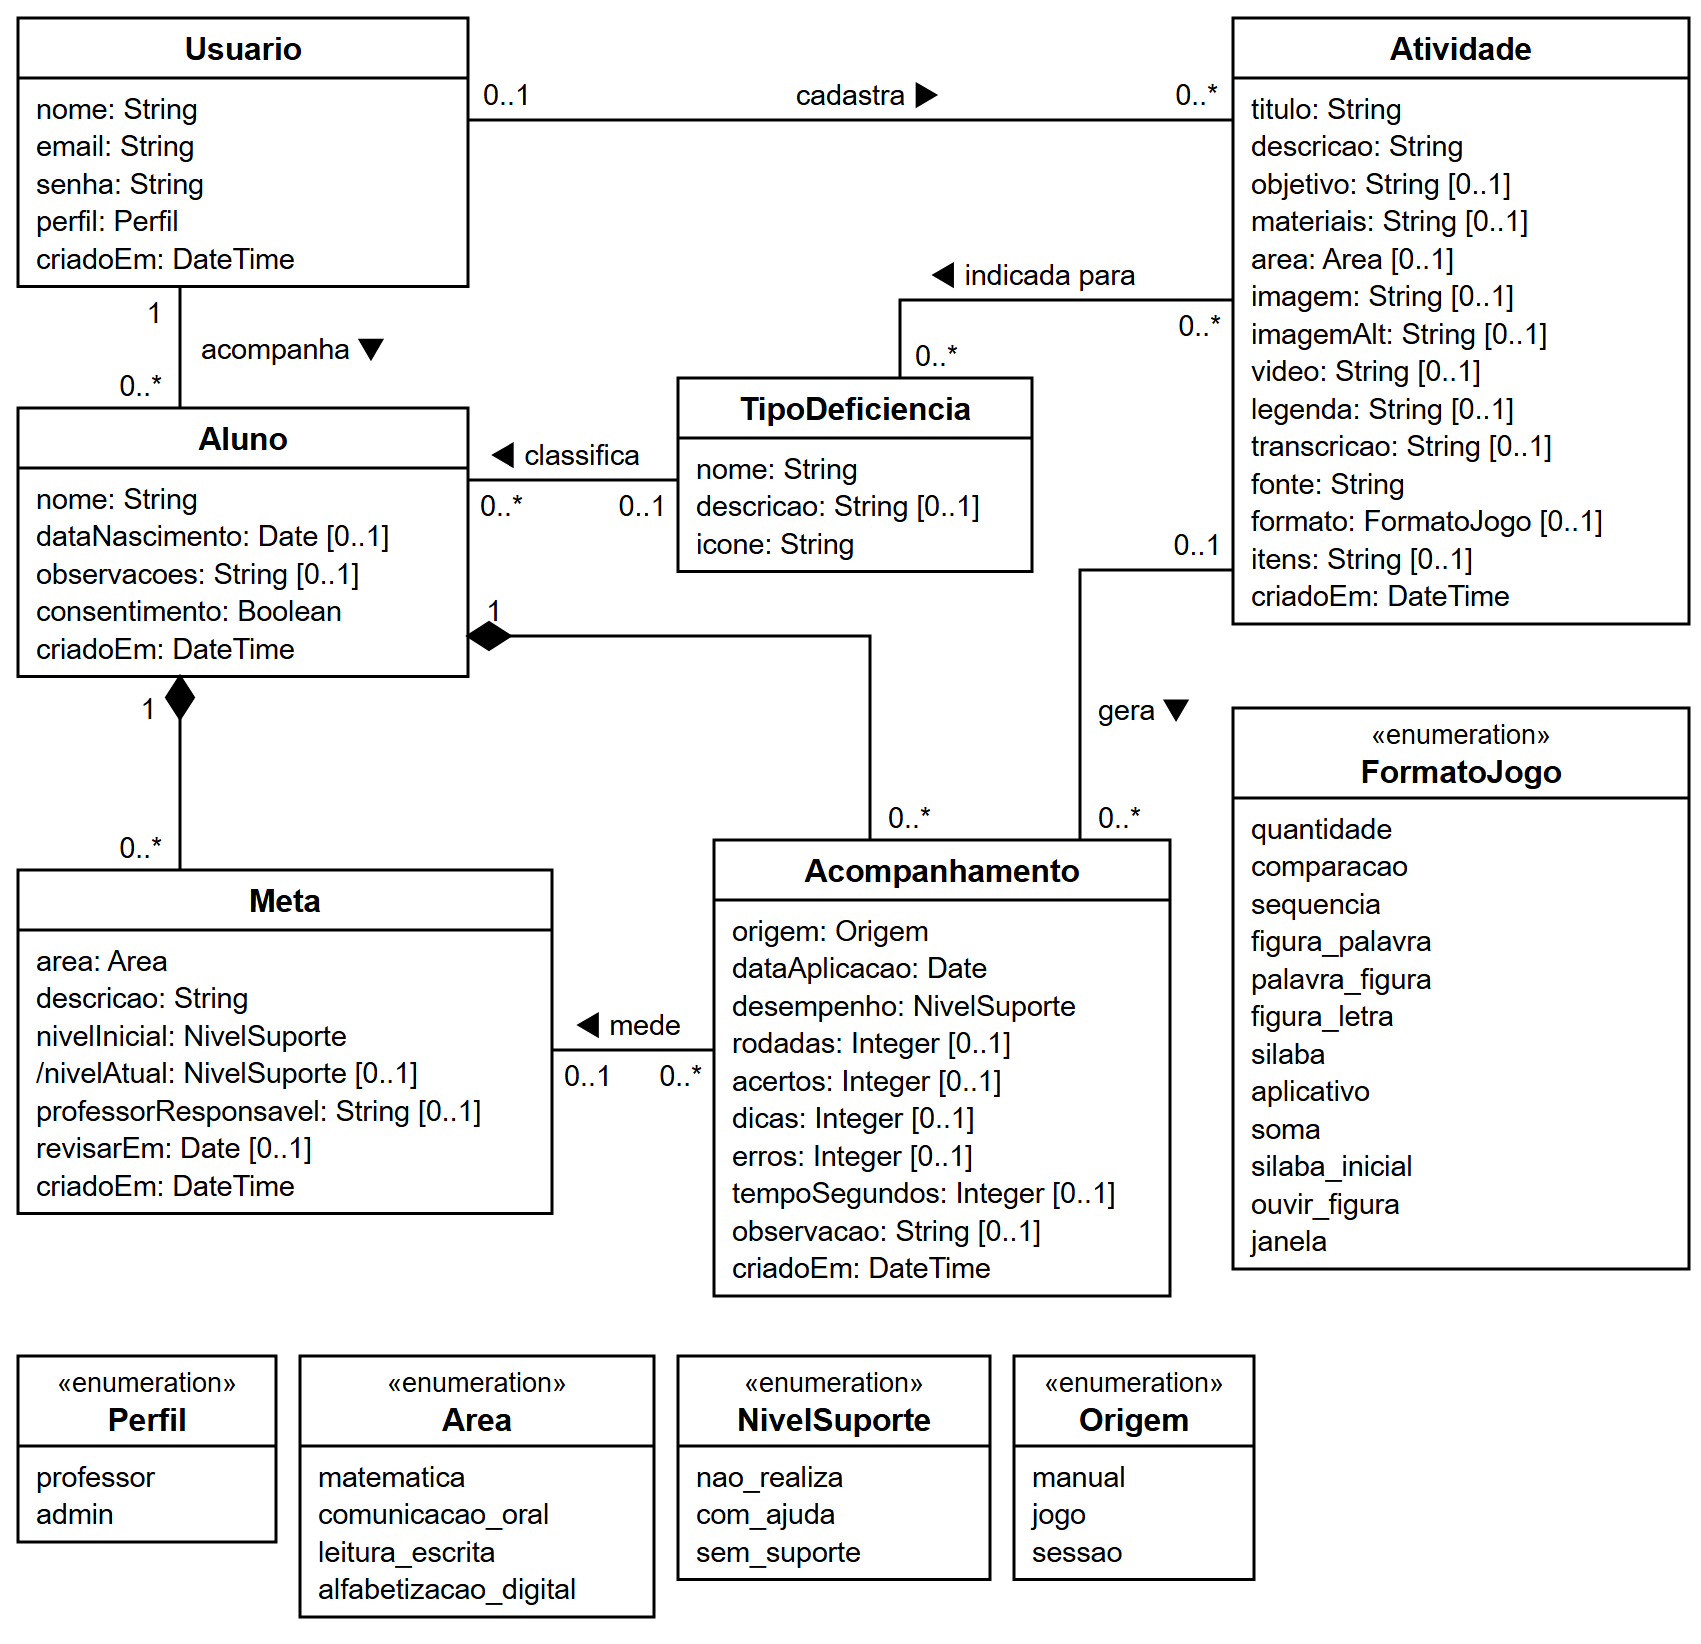
\includegraphics[width=15cm,height=17cm,keepaspectratio]{figuras/figura03-classes.png}
  \fonte{elaboração própria (2026).}
\end{figure}

Na notação da UML (OBJECT MANAGEMENT GROUP, 2017, p. 113, 168, 201 e 202), cada classe tem o nome no primeiro compartimento e os atributos no segundo, na forma nome: Tipo. A multiplicidade [0..1] indica atributo opcional, e a barra antes de \textit{nivelAtual} indica atributo derivado: o nível atual da meta é calculado a partir do registro mais recente. As associações são linhas contínuas com a multiplicidade em cada ponta, e o triângulo junto ao nome dá o sentido da leitura, como em “\textit{Usuario} cadastra \textit{Atividade}”. O losango preto marca a composição: metas e acompanhamentos pertencem a um único aluno e, no sistema, são apagados junto com ele. As cinco enumerações, marcadas com «enumeration», listam os valores aceitos pelos atributos de perfil, área, nível de suporte, origem e formato do jogo; em \textit{Origem}, os valores \textit{manual} e \textit{jogo} só existem por compatibilidade com bancos de versões anteriores, e o sistema atual grava apenas \textit{sessao}. As operações foram omitidas, porque o diagrama descreve os dados do domínio.

\section{Mini games e sessão de atividades}\label{sec:4.4}

Cada atividade do catálogo pertence a uma das quatro áreas e usa um dos 12 formatos de mini game. As rodadas são sorteadas a partir de um catálogo de 14 figuras desenhadas em SVG pelo próprio sistema (bola, bolo, carro, casa, copo, estrela, flor, gato, livro, lua, maçã, pato, peixe e sol), sem arquivos de imagem nem acesso à internet. Cada figura guarda a palavra, a letra inicial e a divisão em sílabas, como ES-TRE-LA, e tem silhueta própria, para que nenhuma informação dependa de cor. O Quadro~\ref{qua:6} descreve os formatos e indica as habilidades da Base Nacional Comum Curricular (BNCC) que cada um exercita.

\begin{tabelaIFTO}
\setlength{\largtab}{\dimexpr\linewidth-8\tabcolsep-5\arrayrulewidth-1pt\relax}
\begin{longtable}{|L{0.1895}|L{0.3499}|L{0.2508}|L{0.2099}|}
\legendatab{quadro}{Formatos de mini game}{qua:6}{4}\\
\hline
\textbf{Formato} & \textbf{O que aparece na tela} & \textbf{Área} & \textbf{BNCC (1º ano)} \\
\hline
\endfirsthead
\multicolumn{4}{@{}r@{}}{\textit{(continuação)}}\\
\hline
\textbf{Formato} & \textbf{O que aparece na tela} & \textbf{Área} & \textbf{BNCC (1º ano)} \\
\hline
\endhead
\multicolumn{4}{@{}r@{}}{\textit{(continua)}}\\
\endfoot
\fontetab{4}{elaboração própria (2026), com as habilidades de Brasil (2018b).}
\endlastfoot
Contar & Figuras repetidas para contar; o aluno escolhe entre todos os numerais, de 1 ao maior número da atividade & Alfabetização Matemática & EF01MA01, EF01MA02 \\ \hline
Comparar & Dois grupos de figuras; o aluno escolhe o que tem mais, ou menos & Alfabetização Matemática & EF01MA03 \\ \hline
Sequência & Sequência de numerais com uma lacuna e três numerais para completá-la & Alfabetização Matemática & EF01MA10 \\ \hline
Juntar & Dois grupos de figuras iguais; o aluno escolhe o total entre três numerais & Alfabetização Matemática & EF01MA06, EF01MA08 \\ \hline
Figura e palavra & Uma figura e três palavras & Leitura e Escrita & EF12LP01 \\ \hline
Palavra e figura & Uma palavra escrita e três figuras & Leitura e Escrita & EF12LP01 \\ \hline
Letra inicial & Uma figura e três letras & Leitura e Escrita & EF01LP07 \\ \hline
Sílaba inicial & Uma figura e três sílabas & Leitura e Escrita & EF01LP08, EF01LP09 \\ \hline
Sílaba que falta & A figura e o nome com uma sílaba faltando; três sílabas para completar & Leitura e Escrita & EF01LP08, EF01LP13 \\ \hline
Ouvir e escolher & Botão “Ouvir a palavra”, que usa a voz do navegador sem mostrar a palavra escrita, e três figuras & Comunicação Oral & Competência geral 4 \\ \hline
Abrir, usar e fechar & Tablet simulado: abrir o aplicativo pedido entre quatro ícones, usar o jogo de palavras dentro dele em três rodadas e fechá-lo & Alfabetização Digital & Competência geral 5 \\ \hline
Botões da janela & Aplicativo aberto; o aluno toca no botão pedido: Fechar, Minimizar ou Voltar & Alfabetização Digital & Competência geral 5 \\ \hline
\end{longtable}
\end{tabelaIFTO}

A última coluna liga cada formato às habilidades do 1º ano da BNCC. Em Matemática, os jogos trabalham o número como indicador de quantidade e a contagem (EF01MA01 e EF01MA02), a comparação de quantidades para indicar “tem mais” ou “tem menos” (EF01MA03), os fatos básicos da adição e o significado de juntar, com o suporte de imagens (EF01MA06 e EF01MA08), e os elementos ausentes em sequências de números naturais (EF01MA10) (BRASIL, 2018b, p. 279). Em Língua Portuguesa, trabalham a leitura de palavras (EF12LP01), a relação entre fonemas e letras (EF01LP07) e a relação entre sílabas e sua escrita, comparando sílabas iniciais, mediais e finais (EF01LP08, EF01LP09 e EF01LP13) (BRASIL, 2018b, p. 99, 101). Os jogos de Comunicação Oral não têm habilidade específica do 1º ano e se ligam à competência geral 4, que trata do uso de diferentes linguagens, entre elas a oral; os de Alfabetização Digital se ligam à competência geral 5, que trata de compreender e utilizar tecnologias digitais (BRASIL, 2018b, p. 9). A correspondência é parcial: cada mini game exercita uma parte da habilidade, em formato de múltipla escolha, e não substitui o trabalho do professor com ela.

Um campo opcional de configuração, gravado em JSON na atividade, permite que um mesmo formato gere atividades diferentes. A chave \textit{figuras} restringe as figuras sorteadas, por exemplo a palavras parecidas como bola, bolo, gato e pato; a chave \textit{app} escolhe o aplicativo do tablet simulado; e a chave \textit{maximo}, de 2 a 10, define o maior número dos jogos de matemática. É assim que existem, por exemplo, “Contar e escolher o numeral (até 5)” e “(até 10)”.

O catálogo inicial tem 24 atividades, seis por área, listadas no Quadro~\ref{qua:7}. Seis atividades por área permitem variar o exercício e a dificuldade dentro de uma mesma meta. Todas foram propostas neste projeto e ainda não passaram por validação de profissionais da educação especial.

\begin{tabelacurta}
\setlength{\largtab}{\dimexpr\linewidth-4\tabcolsep-3\arrayrulewidth-1pt\relax}
\legenda{quadro}{Atividades iniciais do catálogo, por área}\label{qua:7}\vspace{4pt}
\begin{tabular}{|L{0.3571}|L{0.6429}|}
\hline
\textbf{Área} & \textbf{Atividades} \\
\hline
Alfabetização Matemática & Contar e escolher o numeral (até 5); Contar e escolher o numeral (até 10); Comparar quantidades: mais e menos (até 5); Comparar quantidades: mais e menos (até 10); Completar a sequência de numerais (até 10); Juntar quantidades (até 5) \\ \hline
Leitura e Escrita & Associar figura e palavra; Associar figura e palavra: palavras parecidas; Ler a palavra e escolher a figura; Identificar a letra inicial da figura; Identificar a sílaba inicial da figura; Completar a sílaba que falta \\ \hline
Comunicação Oral & Ouvir a palavra e escolher a figura; Ouvir e escolher: animais; Ouvir e escolher: céu e natureza; Ouvir e escolher: objetos; Ouvir e escolher: coisas da mesa; Ouvir e escolher: palavras parecidas \\ \hline
Alfabetização Digital & Abrir, usar e fechar: Palavras e figuras; Abrir, usar e fechar: Calendário; Abrir, usar e fechar: Relógio; Abrir, usar e fechar: Fotos; Abrir, usar e fechar: Música; Botões da janela: fechar, minimizar e voltar \\ \hline
\end{tabular}
\fonte{elaboração própria (2026).}
\end{tabelacurta}

As atividades estão ligadas a todos os tipos de deficiência, com duas exceções. Nenhuma está ligada à deficiência visual, porque todas dependem de ver as figuras, e as de ouvir a palavra não estão ligadas à deficiência auditiva. Essa ligação é usada nas sugestões de atividades para cada meta.

A sessão de atividades é o caminho em que o aluno responde e o resultado é medido sem digitação do professor. A Figura~\ref{fig:4} mostra, num diagrama de sequência da UML, a troca de mensagens entre os participantes de uma sessão.

\begin{figure}[hbp]
  \legendafig{figure}{Diagrama de sequência da sessão de mini games}{fig:4}
  % Diagrama de sequência da UML com Professor, Aluno, SessaoController, SessaoAtividade e Acompanhamento e os fragmentos loop, opt e alt
  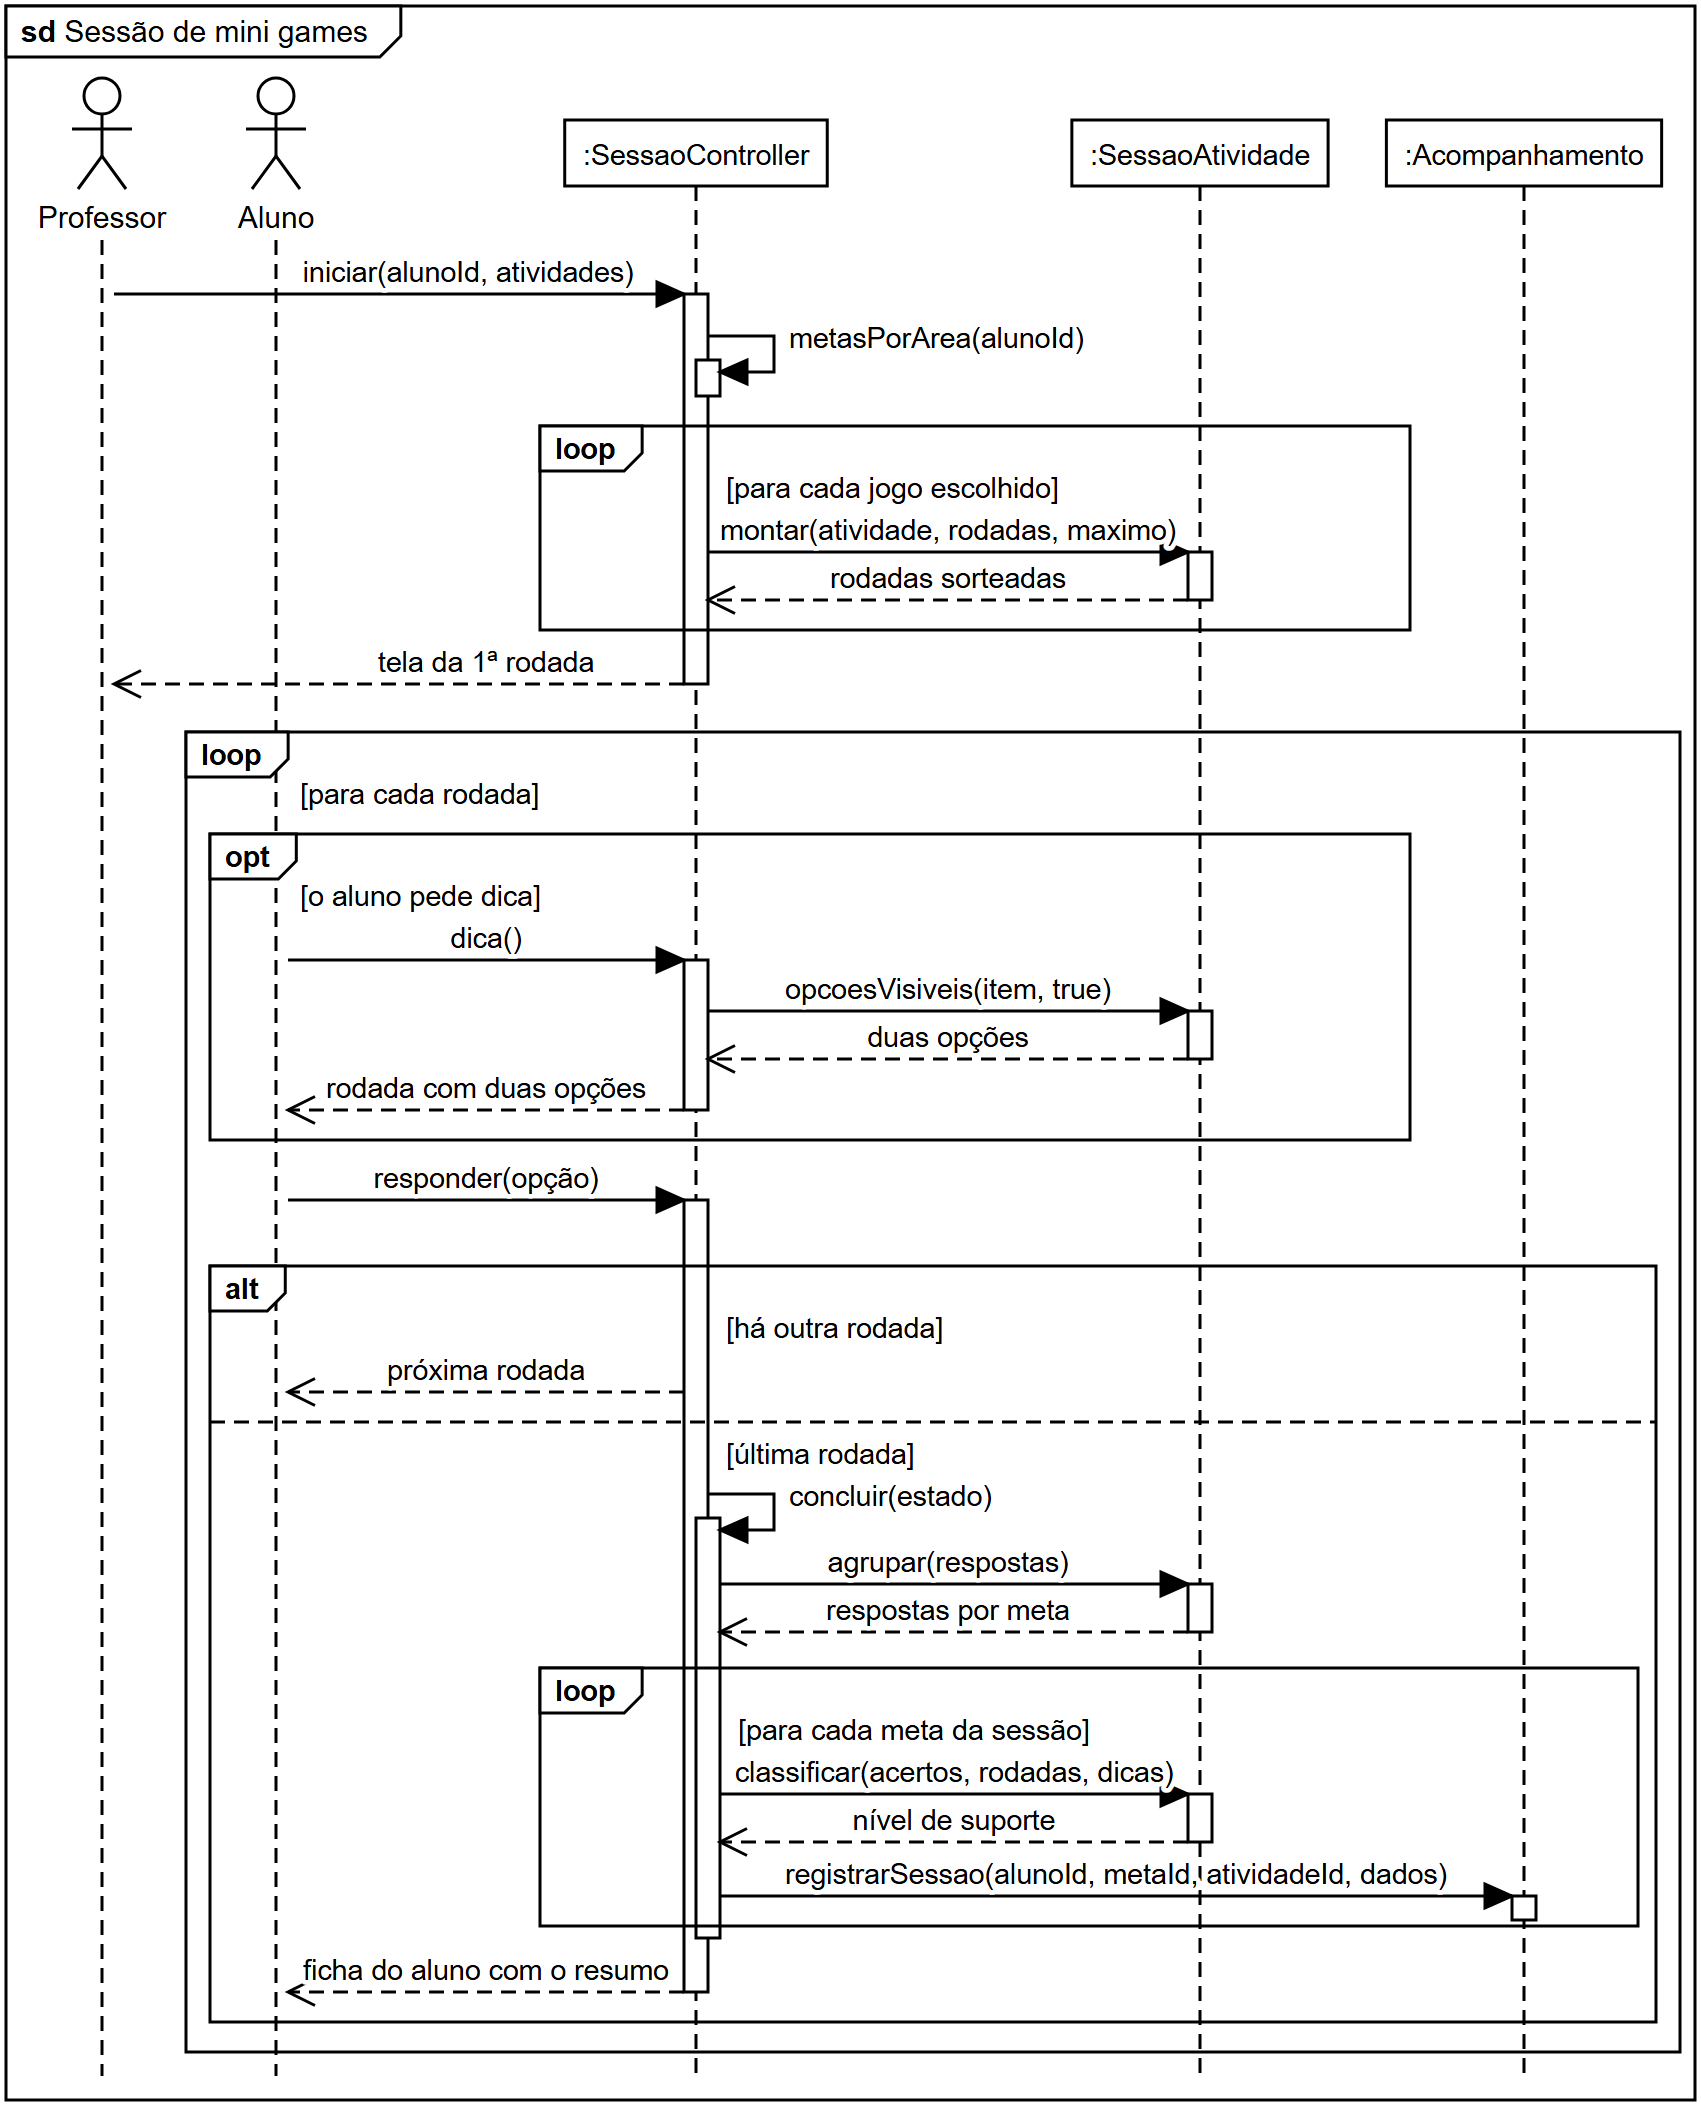
\includegraphics[width=15cm,height=17cm,keepaspectratio]{figuras/figura04-sequencia.png}
  \fonte{elaboração própria (2026).}
\end{figure}

Na Figura~\ref{fig:4}, cada participante tem uma linha de vida tracejada: o professor e o aluno, como atores, e três objetos do sistema, o controlador da sessão (\textit{SessaoController}), o serviço que monta e classifica as rodadas (\textit{SessaoAtividade}) e o modelo que grava os registros (\textit{Acompanhamento}). O banco de dados não aparece, porque não é um objeto da aplicação: a gravação é feita dentro do modelo. A moldura com o rótulo sd delimita a interação; as setas de ponta cheia são chamadas, as tracejadas são retornos, e os retângulos estreitos sobre as linhas de vida mostram quando cada objeto está em execução (OBJECT MANAGEMENT GROUP, 2017, p. 568 e 577). A seta que volta para o próprio controlador, como em \textit{metasPorArea(alunoId)}, é uma chamada a si mesmo; essa, logo no início, escolhe a meta em que cada área será registrada.

Os retângulos com um nome no canto superior esquerdo são fragmentos combinados. O operador do canto diz o que acontece com as mensagens de dentro, e a condição entre colchetes, chamada guarda, diz quando acontece; a guarda fica junto à linha de vida do primeiro evento do fragmento (OBJECT MANAGEMENT GROUP, 2017, p. 583-585). A Figura~\ref{fig:4} tem cinco fragmentos, de três tipos:

\begin{alineasIFTO}
  \item loop [para cada jogo escolhido], no início da Figura~\ref{fig:4}: repete a chamada \textit{montar(atividade, rodadas, maximo)} uma vez para cada jogo marcado pelo professor; cada repetição devolve as cinco rodadas sorteadas daquele jogo, e as rodadas de todos os jogos formam a sessão;
  \item loop [para cada rodada], que ocupa a maior parte da Figura~\ref{fig:4}: repete, rodada a rodada, a troca entre o aluno e o sistema, com o pedido opcional de dica, a resposta e a conferência; o laço termina na última rodada;
  \item opt [o aluno pede dica], dentro do loop das rodadas: o trecho só acontece quando o aluno toca em “Pedir dica”; então o controlador pede ao serviço as opções da rodada com a dica, \textit{opcoesVisiveis(item, true)}, e a rodada volta com duas opções; sem o pedido, nada do que está dentro do opt acontece, e a rodada segue com todas as opções;
  \item alt [há outra rodada] e [última rodada], logo depois da conferência da resposta: executa um dos dois trechos separados pela linha tracejada; se há outra rodada, o aluno recebe a próxima; na última, o controlador executa \textit{concluir(estado)}, pede ao serviço que agrupe as respostas por meta e devolve a ficha do aluno com o resumo;
  \item loop [para cada meta da sessão], dentro do segundo trecho do alt: para cada meta que teve jogos na sessão, classifica o nível de suporte com \textit{classificar(acertos, rodadas, dicas)} e grava um registro com \textit{registrarSessao(alunoId, metaId, atividadeId, dados)}.
\end{alineasIFTO}

O professor inicia a sessão e entrega o aparelho ao aluno; por isso a primeira rodada volta ao professor, e a ficha, resposta à última rodada, aparece no mesmo aparelho. O botão Cancelar, que encerra a sessão sem gravar, não foi representado.

A sessão segue seis passos:

\begin{passos}
  \item Na ficha do aluno, o professor marca um ou mais jogos, ou usa o botão “Fazer na tela” de uma sugestão, que já indica a meta. Sem indicação, cada jogo vai para a primeira meta do aluno na mesma área, mostrada ao lado do jogo; os jogos de áreas sem meta ficam desabilitados.
  \item O sistema sorteia cinco rodadas por jogo. No formato de aplicativo, as cinco rodadas são as etapas: abrir, três rodadas de uso e fechar.
  \item A tela mostra uma rodada por vez, com o enunciado, uma cena desenhada e botões grandes; um toque já responde. Essa tela não traz o menu do professor, para que a criança não saia do jogo por engano; só o botão Cancelar, que pede confirmação, encerra a sessão antes do fim.
  \item O aluno pode pedir uma dica por rodada. Nas rodadas com três ou mais opções, a dica deixa apenas duas, a correta e uma errada, numa ordem que não revela qual é a certa. No jogo de comparar, que já tem só duas opções, a dica não é oferecida.
  \item Cada resposta é conferida no servidor e guardada com o acerto, o uso de dica e os segundos passados desde a resposta anterior.
  \item Ao final, as respostas são somadas por meta, cada meta recebe um nível de suporte e um registro é gravado para cada meta, com o detalhe por jogo. Cancelar a sessão encerra tudo sem gravar.
\end{passos}

No formato de aplicativo, as três etapas são registradas à parte, e o tempo até o aluno abrir o aplicativo aparece no detalhe do registro.

\section{Classificação e indicadores de evolução}\label{sec:4.5}

Ao fim da sessão, o resultado de cada meta é classificado em um dos três níveis do AppPEI pela regra do Quadro~\ref{qua:8}.

\begin{tabelacurta}
\setlength{\largtab}{\dimexpr\linewidth-4\tabcolsep-3\arrayrulewidth-1pt\relax}
\legenda{quadro}{Regra de classificação do nível de suporte}\label{qua:8}\vspace{4pt}
\begin{tabular}{|L{0.5924}|L{0.4076}|}
\hline
\textbf{Resultado da sessão na meta} & \textbf{Nível registrado} \\
\hline
Nenhum acerto & Não realiza \\ \hline
Todas as rodadas certas, sem nenhuma dica & Realiza sem necessidade de suporte \\ \hline
Qualquer outro caso: acertos parciais, ou todos certos com dica & Realiza com ajuda \\ \hline
\end{tabular}
\fonte{elaboração própria (2026), com os níveis de Francisco (2023).}
\end{tabelacurta}

A regra exige a evidência mais forte para o nível mais alto: acertar tudo sem nenhum apoio. Ela é uma hipótese do protótipo (seção~\ref{sec:5.4}). Um ponto a discutir com professores é que o nível “realiza com ajuda” reúne duas situações diferentes: o aluno que usou dica e o aluno que não usou dica, mas errou alguma rodada.

Com as sessões de uma meta em ordem cronológica, o sistema calcula quatro indicadores:

\begin{alineasIFTO}
  \item acerto médio: total de acertos dividido pelo total de rodadas, em porcentagem;
  \item autonomia: porcentagem de sessões classificadas como “realiza sem necessidade de suporte”;
  \item sessões com dica: porcentagem de sessões em que houve pelo menos uma dica;
  \item variação: diferença, em pontos percentuais, entre o acerto médio da segunda e o da primeira metade das sessões, a partir de seis sessões.
\end{alineasIFTO}

Sendo $t_i$ a taxa de acerto da sessão $i$ ($\mathit{acertos} \div \mathit{rodadas} \times 100$), $n$ o número de sessões e $m$ a metade de $n$ arredondada para baixo, a variação é:

\begin{equation}
\Delta = \frac{1}{m}\sum_{i=n-m+1}^{n} t_i \;-\; \frac{1}{m}\sum_{i=1}^{m} t_i, \qquad m = \left\lfloor \frac{n}{2} \right\rfloor, \quad n \geq 6
\label{eq:variacao}
\end{equation}

Quando $n$ é ímpar, a sessão do meio fica fora das duas médias. O mínimo de seis sessões evita que cada metade tenha uma ou duas sessões, caso em que um único dia atípico mudaria o resultado. A Tabela~\ref{tab:1} mostra um exemplo com dados fictícios.

\begin{tabelacurta}
\setlength{\largtab}{\dimexpr\linewidth-10\tabcolsep-0\arrayrulewidth-1pt\relax}
\legenda{table}{Exemplo fictício de seis sessões de uma meta}\label{tab:1}\vspace{4pt}
\begin{tabular}{C{0.0982}C{0.2223}C{0.0858}C{0.1603}L{0.4334}}
\hline
\textbf{Sessão} & \textbf{Acertos (de 5)} & \textbf{Dicas} & \textbf{Acerto (\%)} & \textbf{Nível registrado} \\
\hline
1 & 2 & 2 & 40,0 & Realiza com ajuda \\
2 & 2 & 1 & 40,0 & Realiza com ajuda \\
3 & 3 & 1 & 60,0 & Realiza com ajuda \\
4 & 4 & 1 & 80,0 & Realiza com ajuda \\
5 & 4 & 0 & 80,0 & Realiza com ajuda \\
6 & 5 & 0 & 100,0 & Realiza sem necessidade de suporte \\
\hline
\end{tabular}
\fonte{elaboração própria (2026), com dados fictícios.}
\end{tabelacurta}

No exemplo, o acerto médio é 66,7\% (20 acertos em 30 rodadas), a autonomia é 16,7\% (uma sessão em seis) e as sessões com dica são 66,7\% (quatro em seis). A média da primeira metade é 46,7\% e a da segunda, 86,7\%, o que dá uma variação de +40,0 pontos percentuais. A sessão 5 mostra a nuance da regra: sem dica, mas com um erro, ela ainda é registrada como “realiza com ajuda”.

\section{Gráficos de evolução}\label{sec:4.6}

Na ficha do aluno, a seção “Evolução nas sessões na tela” mostra uma tabela com os indicadores de cada meta e, para cada meta com sessões, um cartão com dois gráficos desenhados em SVG pelo servidor, sem biblioteca externa. A Figura~\ref{fig:5} reproduz esse cartão para os dados da Tabela~\ref{tab:1}; ela foi gerada com as mesmas classes que o sistema usa na ficha, alimentadas com os dados fictícios do exemplo.

\begin{figure}[hbp]
  \legendafig{figure}{Gráficos de evolução gerados pelo UNIA para os dados da Tabela 1}{fig:5}
  % Linha do acerto nas seis sessões, de 40% a 100%, com as médias tracejadas de 46,7% e 86,7% e a linha do tempo do nível de suporte
  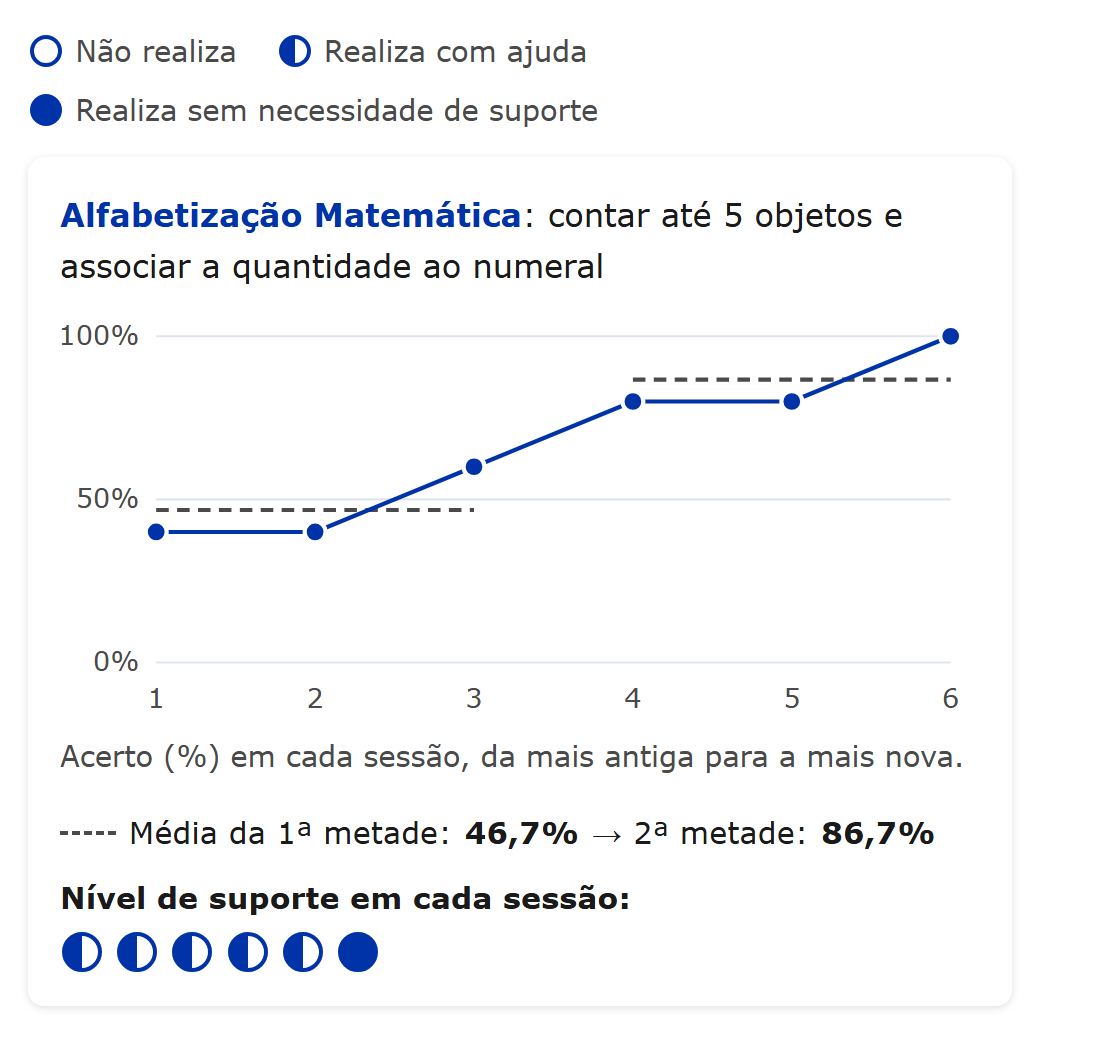
\includegraphics[width=14.5cm,height=17cm,keepaspectratio]{figuras/figura05-graficos-evolucao.png}
  \fonte{elaboração própria (2026), com dados fictícios.}
\end{figure}

O primeiro gráfico é uma linha com a taxa de acerto de cada sessão, da mais antiga para a mais nova. A partir de seis sessões, duas linhas tracejadas mostram a média de cada metade, e a distância vertical entre elas é a variação; os valores das médias aparecem em texto abaixo do gráfico, para não cobrir os pontos. Ao passar o mouse sobre um ponto, o sistema mostra a data, os acertos e as dicas daquela sessão.

O segundo gráfico é uma linha do tempo do nível de suporte, com um símbolo por sessão: círculo vazio para “não realiza”, meio cheio para “realiza com ajuda” e cheio para “realiza sem necessidade de suporte”. Como a forma muda, e não apenas a cor, o nível pode ser lido sem depender da percepção de cores. Cada gráfico tem também uma descrição em texto, lida por leitores de tela, com os valores de todas as sessões e as médias, e os números exatos continuam na tabela da ficha.

\section{Segurança e privacidade}\label{sec:4.7}

O UNIA guarda dados de crianças, e parte deles, como o tipo de deficiência e o estudo de caso, pode ser considerada dado referente à saúde, que a Lei Geral de Proteção de Dados Pessoais (LGPD) classifica como dado pessoal sensível (BRASIL, 2018a, art. 5º, II). A mesma lei exige que o tratamento de dados de crianças atenda ao seu melhor interesse e conte com o consentimento específico de pelo menos um dos pais ou do responsável legal (BRASIL, 2018a, art. 14). Por isso, a segurança foi tratada como requisito desde a versão 2. O Quadro~\ref{qua:9} relaciona as ameaças consideradas, baseadas nas categorias do Top 10 do Open Worldwide Application Security Project (OWASP), lista dos riscos mais críticos de segurança em aplicações web (OWASP FOUNDATION, 2021), aos mecanismos adotados.

\begin{tabelaIFTO}
\setlength{\largtab}{\dimexpr\linewidth-4\tabcolsep-3\arrayrulewidth-1pt\relax}
\begin{longtable}{|L{0.4043}|L{0.5957}|}
\legendatab{quadro}{Ameaças e mecanismos de segurança}{qua:9}{2}\\
\hline
\textbf{Ameaça} & \textbf{Mecanismo no UNIA} \\
\hline
\endfirsthead
\multicolumn{2}{@{}r@{}}{\textit{(continuação)}}\\
\hline
\textbf{Ameaça} & \textbf{Mecanismo no UNIA} \\
\hline
\endhead
\multicolumn{2}{@{}r@{}}{\textit{(continua)}}\\
\endfoot
\fontetab{2}{elaboração própria (2026).}
\endlastfoot
Vazamento de senhas do banco & Senhas guardadas com \textit{password\_hash()} e conferidas com \textit{password\_verify()} \\ \hline
Injeção de SQL & PDO com consultas parametrizadas e emulação de prepared statements desligada \\ \hline
Script injetado na página (XSS) & Escape de toda saída de dado digitado pelo usuário \\ \hline
Formulário forjado (CSRF) & Token por sessão, conferido pelo roteador em todo POST \\ \hline
Acesso sem login ou sem o perfil exigido & Verificações de acesso nas rotas: visitante, logado ou administrador \\ \hline
Acesso a dados de outro professor & Consultas filtradas pelo professor logado; resposta 404 para dados de terceiros \\ \hline
Força bruta no login & Bloqueio de 5 minutos após 5 tentativas erradas, contadas por sessão \\ \hline
Sequestro de sessão & Cookie \textit{HttpOnly} e \textit{SameSite}; novo identificador de sessão no login \\ \hline
Roubo do token de recuperação de senha & Só o hash Secure Hash Algorithm de 256 bits (SHA-256) do token é gravado; uso único; validade de 60 minutos \\ \hline
Envio de arquivo malicioso & Conferência do tipo real do arquivo, limite de 2 MB, nome aleatório e pasta sem execução de PHP \\ \hline
Exposição de arquivos internos e de erros & Apenas a pasta \textit{public} é servida; os erros vão para o log, e a tela mostra mensagem genérica \\ \hline
\end{longtable}
\end{tabelaIFTO}

Na privacidade, além do isolamento entre professores do Quadro~\ref{qua:9}, o cadastro do aluno só é aceito quando o professor confirma ter a autorização do responsável para registrar os dados, e o formulário de atividades orienta a não enviar fotos de crianças sem autorização. A falta de criptografia das observações do estudo de caso está entre as limitações da seção~\ref{sec:5.4}.

\section{Acessibilidade}\label{sec:4.8}

As telas seguem práticas inspiradas na WCAG 2.1 (W3C, 2018): idioma da página definido como português; rótulos em todos os campos; link para pular direto ao conteúdo; foco visível na navegação por teclado; resumo de erros anunciado aos leitores de tela, com link para cada campo; tabelas com legenda e cabeçalhos associados; texto alternativo obrigatório nas imagens das atividades; campos para legenda e transcrição dos vídeos; e respeito à preferência do usuário por menos animação.

Nos mini games, os botões têm pelo menos 44 por 44 pixels, o tamanho mínimo de alvo de toque do critério 2.5.5 da WCAG 2.1 (W3C, 2018), e um toque já responde. Nenhuma informação depende só de cor, como descrito nas seções~\ref{sec:4.4} e~\ref{sec:4.6}. O mini game de ouvir a palavra usa a síntese de fala da Web Speech API, que lê um texto em voz alta com o sintetizador do dispositivo (MOZILLA, 2026); por isso, a voz em português depende do navegador e do sistema.

Há uma escolha com custo. Nas rodadas, as figuras são tratadas como decorativas para os leitores de tela, e os botões recebem rótulos neutros, como “Figura~\ref{fig:1}”, porque dizer o nome da figura entregaria a resposta. Com isso, os mini games não atendem alunos com deficiência visual, limitação discutida na seção~\ref{sec:5.4}.

Como não houve auditoria de acessibilidade (seção~\ref{sec:5.4}), este trabalho afirma que o UNIA segue práticas inspiradas na WCAG 2.1, e não que atende às diretrizes.

\section{Telas do sistema}\label{sec:4.9}

As Figuras~\ref{fig:6} a~\ref{fig:8} mostram telas do UNIA com dados fictícios. A ficha do aluno (Figura~\ref{fig:6}) reúne numa só página o estudo de caso, as metas com o nível atual, a tabela e os gráficos de evolução, as sugestões de atividades, o formulário da sessão e o histórico; a figura mostra o trecho das metas e da evolução. Na rodada (Figura~\ref{fig:7}), a tela mostra o enunciado, a cena desenhada e um botão grande para cada numeral; abaixo dos botões, fora do recorte, ficam “Pedir dica” e “Cancelar”. No formulário da sessão (Figura~\ref{fig:8}), cada jogo indica a meta em que o resultado será gravado, e os jogos de áreas sem meta aparecem desabilitados. O catálogo de atividades, que não aparece nas figuras, permite buscar atividades e filtrá-las por área e por tipo de deficiência.

\begin{figure}[hbp]
  \legendafig{figure}{Ficha do aluno, com metas, indicadores e gráficos}{fig:6}
  % Ficha do aluno com a tabela de metas, os indicadores de evolução e o início do gráfico de uma meta de leitura e escrita
  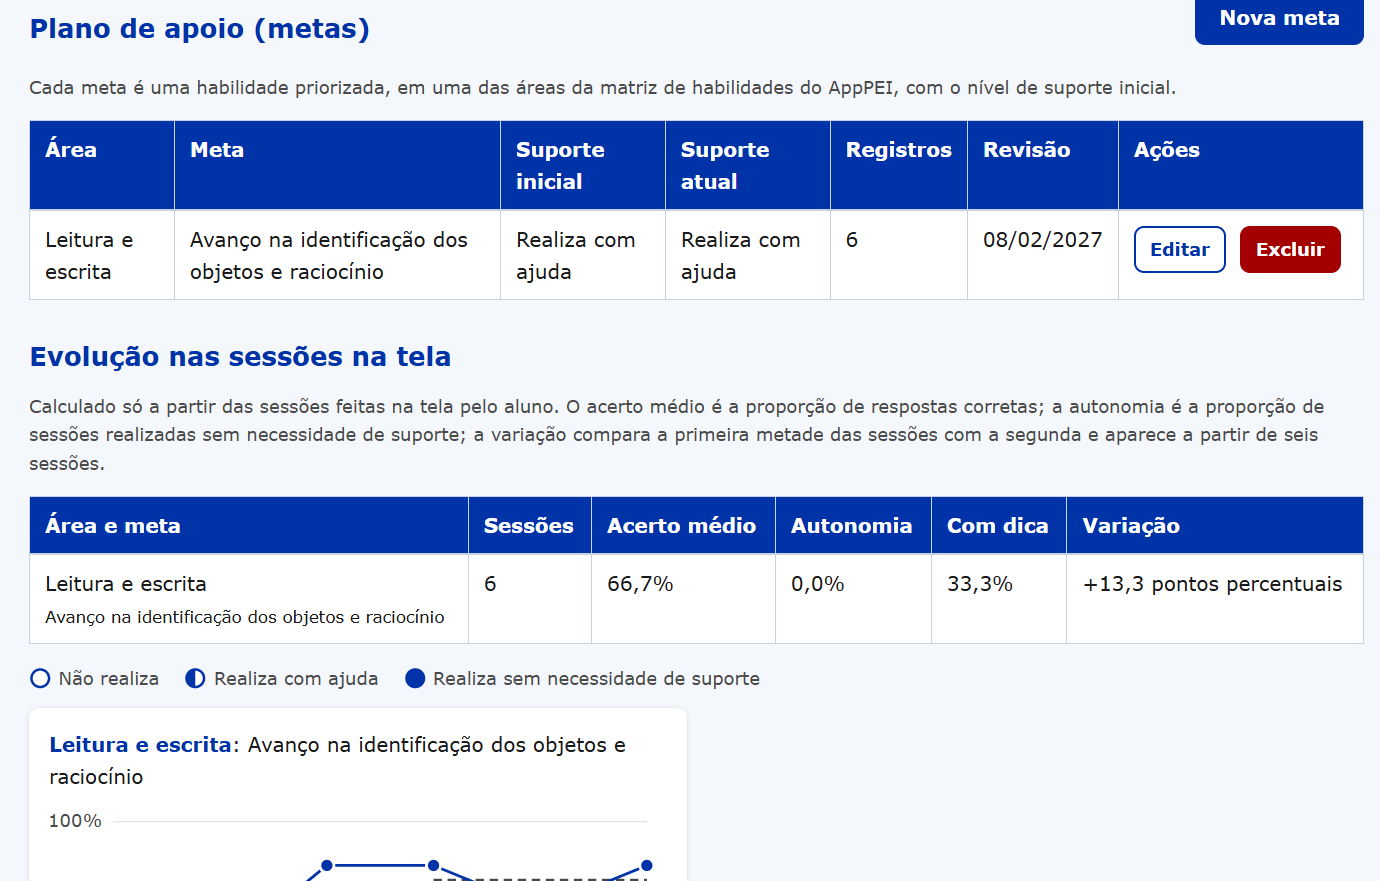
\includegraphics[width=15cm,height=17cm,keepaspectratio]{figuras/figura06-ficha-do-aluno.png}
  \fonte{elaboração própria (2026).}
\end{figure}

\begin{figure}[hbp]
  \legendafig{figure}{Rodada do mini game “Contar e escolher o numeral”}{fig:7}
  % Rodada 2 de 5 do jogo Contar e escolher o numeral até 10: quatro sóis desenhados e botões com os numerais
  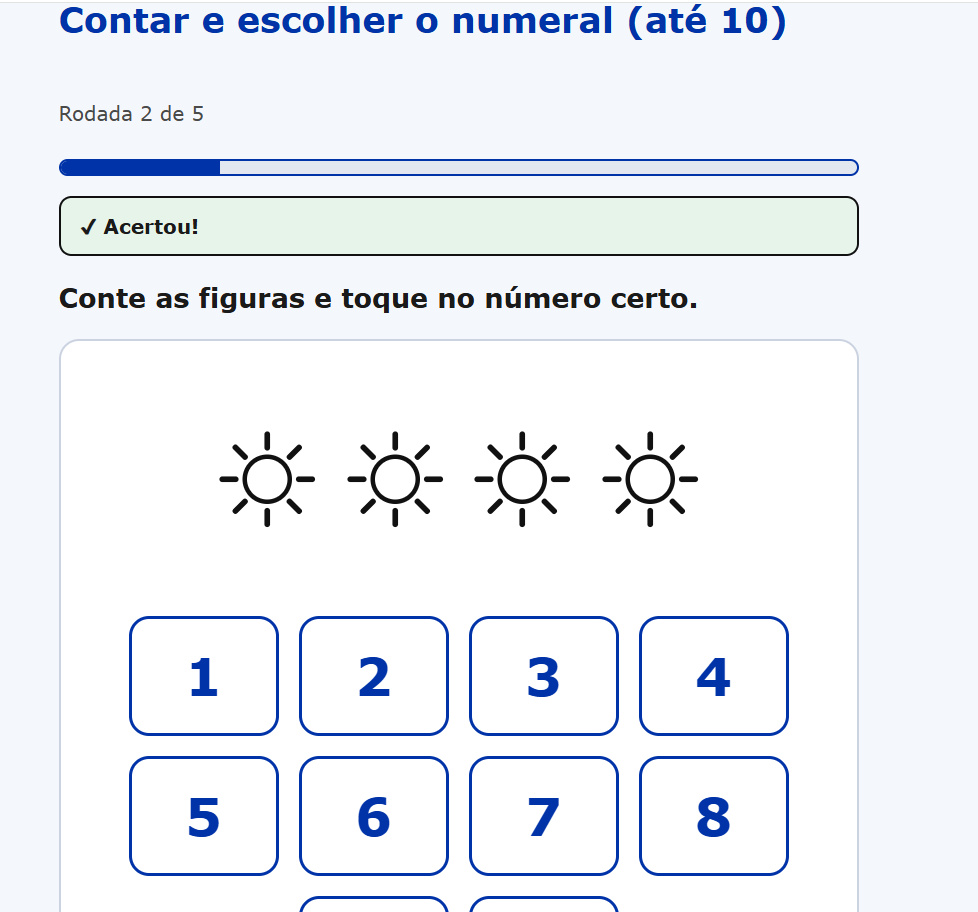
\includegraphics[width=12.9cm,height=10cm,keepaspectratio]{figuras/figura07-rodada.png}
  \fonte{elaboração própria (2026).}
\end{figure}

\begin{figure}[hbp]
  \legendafig{figure}{Escolha dos jogos da sessão, com a meta de cada jogo}{fig:8}
  % Lista de jogos da sessão na ficha do aluno, cada um com a meta em que será gravado; os jogos de áreas sem meta aparecem desabilitados
  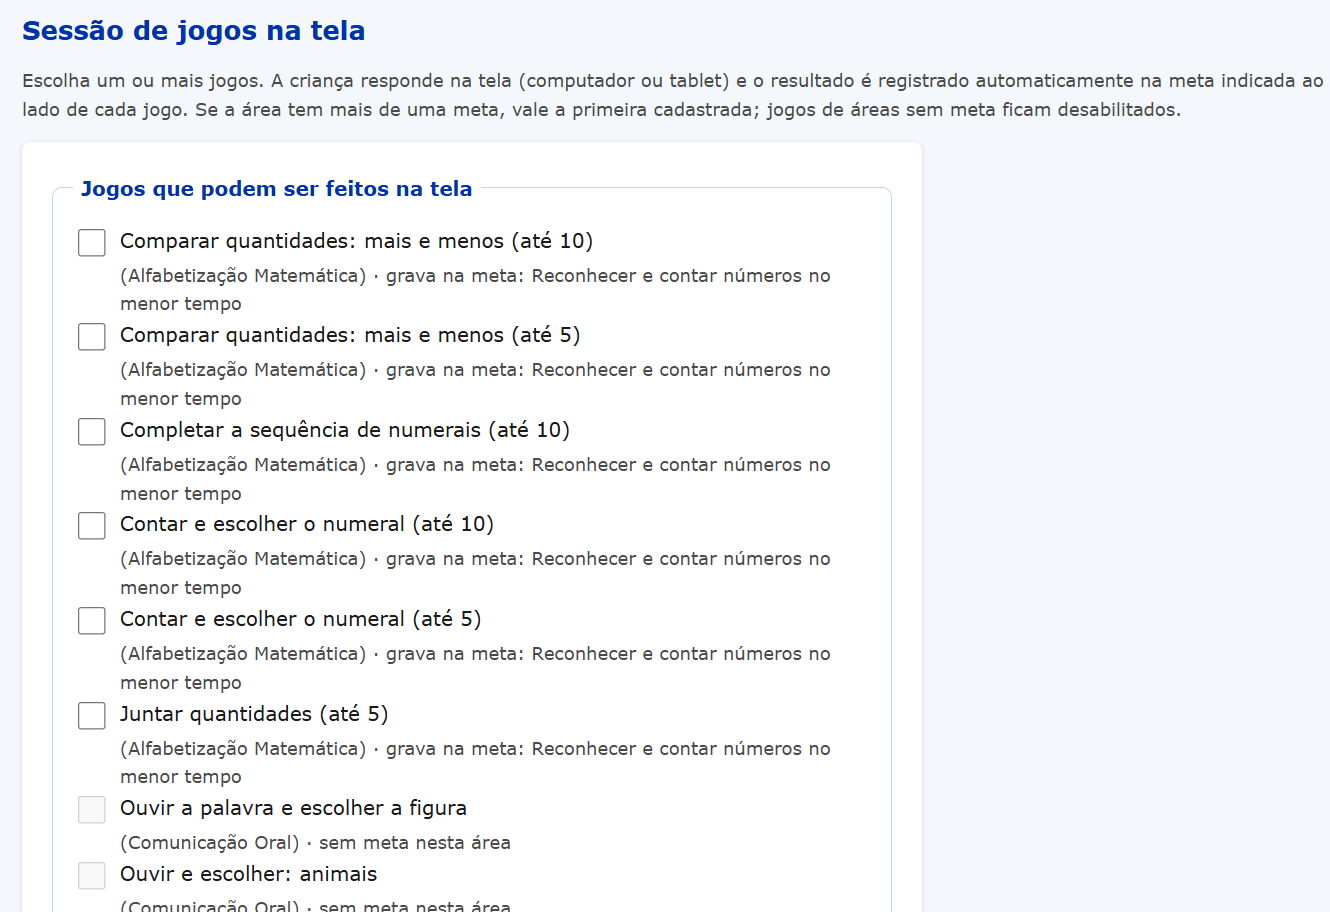
\includegraphics[width=15cm,height=17cm,keepaspectratio]{figuras/figura08-escolha-dos-jogos.png}
  \fonte{elaboração própria (2026).}
\end{figure}
